

\begin{figure}[t!]
    \centering
    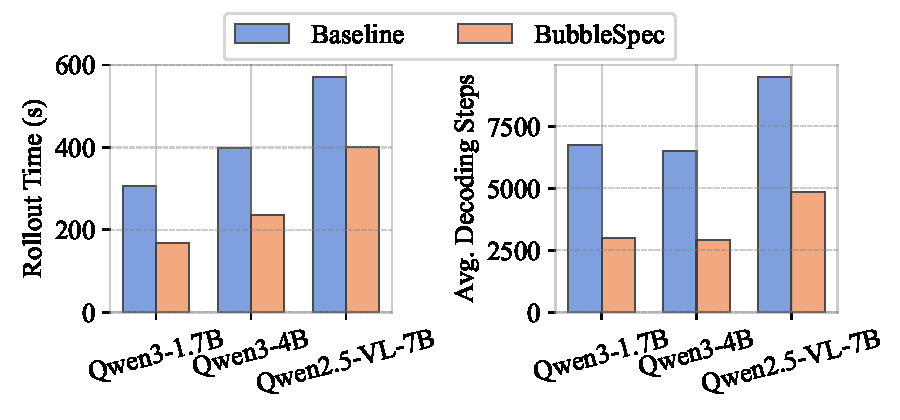
\includegraphics[width=1.0\linewidth]{figures/overall_comp.pdf}
    \caption{BubbleSpec reduces decoding steps by roughly 50\% and delivers up to 1.8× speedup across different models.}
    \label{fig:effect}
\end{figure}

\begin{figure*}[t!]
    \centering
    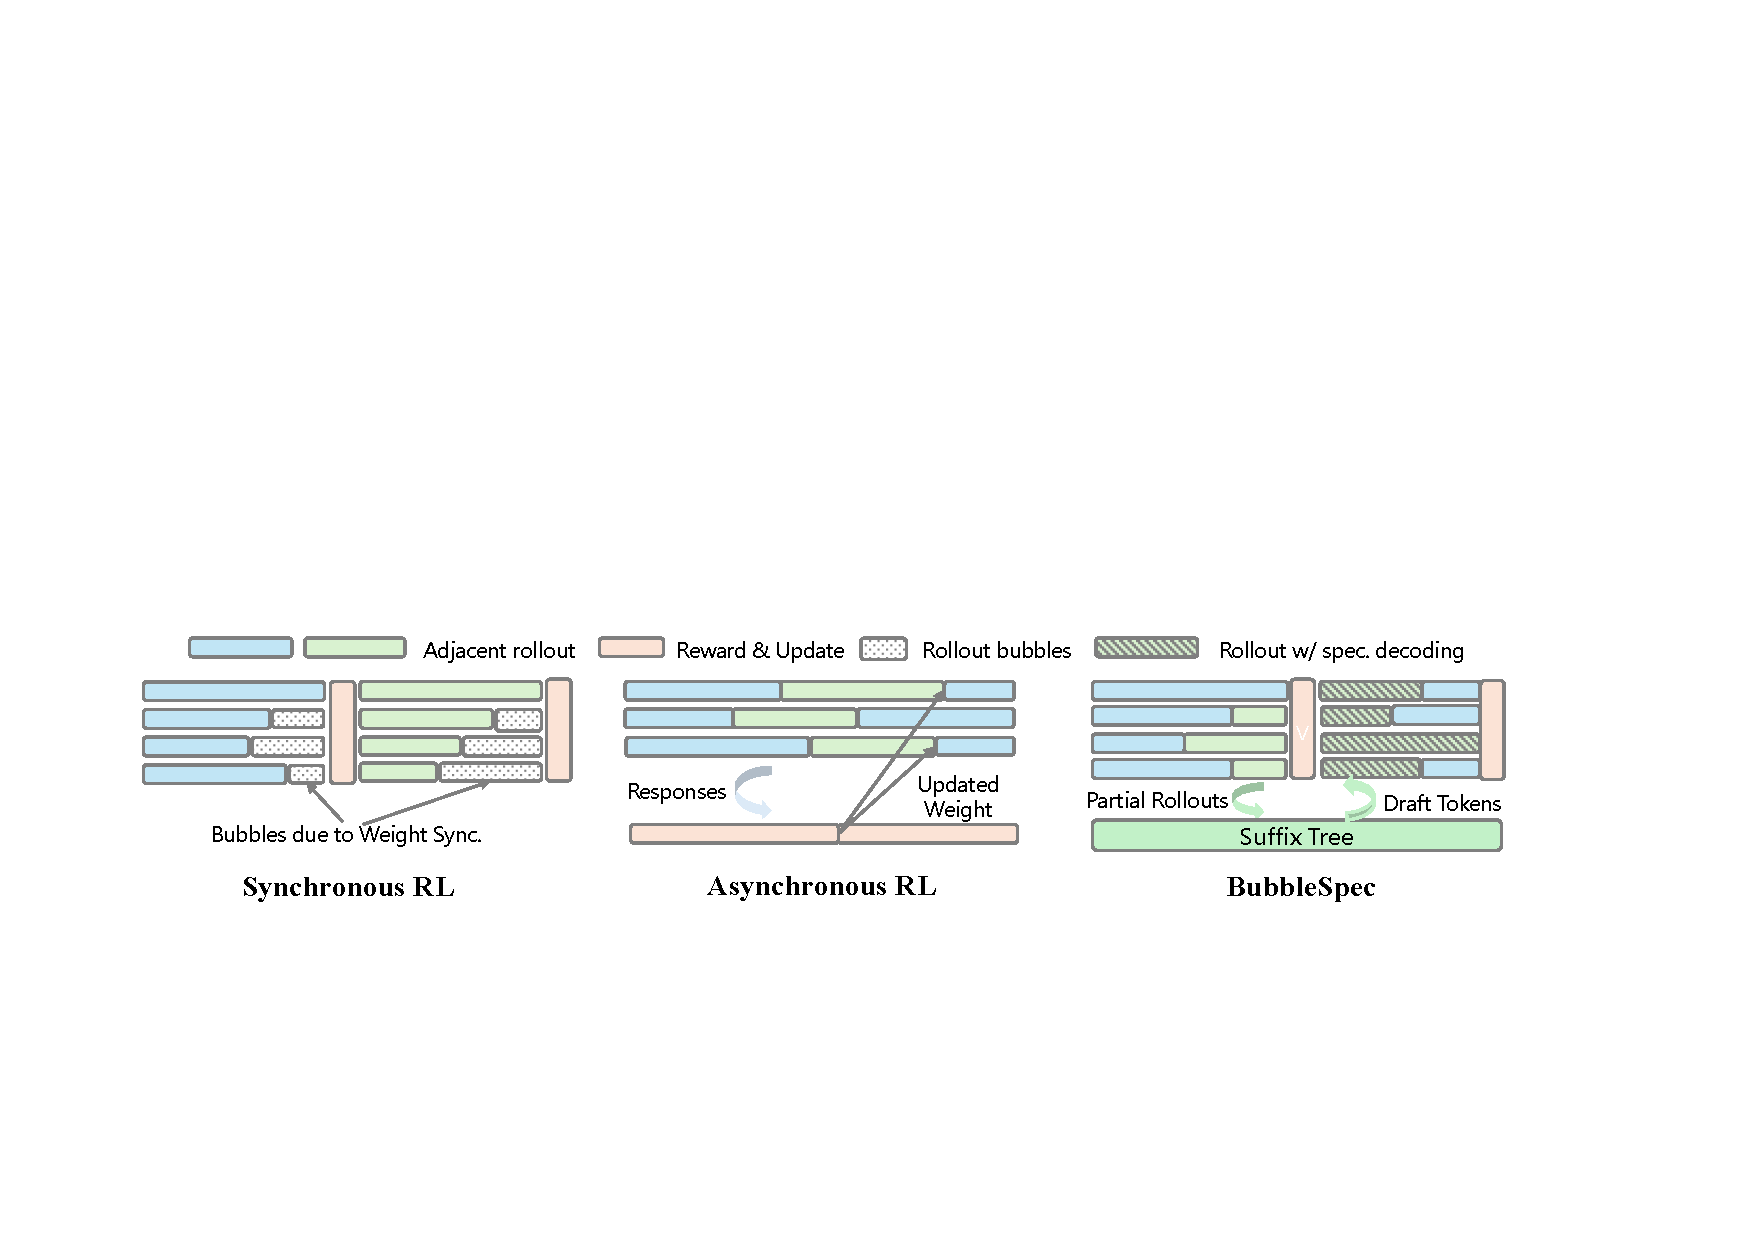
\includegraphics[width=0.95\linewidth]{figures/method_comp.pdf}
    \caption{Compared to existing methods, \model exploits rollout bubbles while maintaining the synchronous nature of RL.}
    \label{fig:rl_workflow}
\end{figure*}
\section{Introduction}

The rapid evolution of Large Language Models (LLMs) has been significantly propelled by Reinforcement Learning (RL)~\cite{ouyang2022training_rlhf, kirk2023understanding}. 
The paradigm of ``test-time scaling'' has emerged as a frontier in enhancing reasoning capabilities, where models are incentivized to generate long Chain-of-Thought (CoT)~\cite{wei2022chain, lyu2023faithful, hu2026smartthinker} reasoning paths to solve complex problems~\cite{snell2024scaling}, represented by works like OpenAI-o1~\cite{jaech2024openai} and DeepSeek-R1~\cite{guo2025deepseek}. In this context, RL plays a pivotal role in discovering and reinforcing these extended reasoning patterns, enabling models to achieve superior performance on mathematical and coding tasks through self-evolution.

However, the efficiency of RL training is largely constrained by the \textit{rollout phase}, where the policy model samples responses for a batch of prompts. The stochastic nature of LLM generation causes unpredictable variance in response lengths, forcing faster devices to idle wait while waiting for stragglers—a phenomenon commonly known as ``bubbles''.
To alleviate the rollout bubble issue, existing approaches~\cite{team2025kimi, zhong2025streamrl} relax the strict synchronization requirement between the rollout and policy update phases, allowing rollout workers to generate sequences continuously without frequent interruptions. 
However, studies~\cite{xi2026jet, qi2025defeating, liuspeed} have shown that such off-policy behavior and rollout--update discrepancies can lead to training instability.

Alternatively, speculative decoding, as a lossless LLM inference acceleration solution, has attracted increasing attention.
In particular, model-free speculative decoding has been a leading option~\cite{he2025history_rhyme, liu2025specRL}, owing to its lightweight draft overhead and the lack of sensitivity to rollout model weight evolution during RL updates. 
These methods typically exploit the strong similarity of responses across adjacent RL training epochs, reusing historical rollout outputs to construct draft candidates for the current batch, thereby accelerating rollouts while preserving the synchronous nature of RL training.


Nevertheless, methods based on cross-epoch response similarity face a fundamental limitation as the training dataset scales up, since they typically require an initial epoch to build a rollout cache for warm-up. 
In modern large-scale training regimes, such as those using DeepMath-103k~\cite{he2025deepmath} and Polaris-53k~\cite{an2025polaris}, a single training epoch may span days to weeks. 
As a result, history-based approaches provide no acceleration during this prolonged initial stage (\ie the \textit{cold-start problem}). Moreover, as the optimization steps within an epoch increase, the policy can evolve substantially, perturbing the distributional similarity between adjacent epochs and reducing the reusability of historical rollouts.

To overcome this limitation, we introduce \textbf{\model}, a synchronous RL framework that fundamentally rethinks how idle time is managed in RL training. As shown in \autoref{fig:rl_workflow}, rather than eliminating bubbles at the cost of losing synchrony, \model strategically \emph{exploits} them through effective cross-step pipelining. 
During the idle window of the current rollout step, it proactively pre-generates rollouts for the next step and organizes the partial responses into a suffix tree that serves as a draft database for speculative decoding at the next step. 
Furthermore, we carefully design our speculative decoding technique, combining it with operator-level optimizations to minimize both draft and verification costs, thereby achieving high end-to-end efficiency for large-batch RL rollouts, a regime where conventional speculative decoding typically fails to provide acceleration.
% Furthermore, we carefully design our speculative decoding technique combining with operator-level optimizations, for minimized draft and verification, achieveing high end-to-end efficiency under large batch size RL rollout. 

% we carefully refine \model's design for realistic system deployments, including reducing rank synchronization latency and suffix-tree construction overhead, as well as operator-level optimizations, to achieve end-to-end efficiency.

We implement \model based on the Verl framework~\cite{sheng2025hybridflow}, and evaluate it in long-context RL scenarios. 
Experimental results show that our \model reduces decoding steps by more than 50\% and improves rollout throughput by up to 1.8$\times$. 
Compared to prior arts, \model offers distinct advantages: 
(1) \textbf{Immediate Acceleration}: It provides speedup from the very first training step, making it uniquely suitable for large-scale dataset training where epoch-based history is unavailable or stale. 
(2) \textbf{Strict Synchronous Guarantee}: By adhering to rigorous speculative decoding protocols, \model ensures the rollout distribution remains mathematically identical to the original policy. 
This allows it to be seamlessly applied to various RL algorithms (\eg GSPO, DAPO, SAPO~\cite{gao2025soft_sapo, yu2025dapo, zheng2025gspo}) without requiring algorithmic modifications or risking performance degradation. In summary, our contributions can be summarized as follows:
\begin{itemize}
    \item We deeply analyze long-tail effects in synchronous RL and highlight key considerations for applying speculative decoding in RL training.
    \item We propose BubbleSpec, the first synchronous RL framework that converts long-tail bubbles into speculative drafts, overcoming the cold-start limitation of history-based approaches.
    \item We design a deployment-oriented speculative decoding scheme that ensures reductions in decoding steps translate into end-to-end efficiency gains.
    \item Extensive evaluations on realistic long-context RL scenarios demonstrate that \model consistently enhances rollout efficiency across various model sizes.
\end{itemize}

\textbf{Conflict of Interest Disclosure.} The authors declare that they have no financial conflicts of interest related to this work.
